\section{Generative Art}
% 		- Art Rules
% 		- 3D Assets
% 			- Furniture
% 			- Props
% 			- Deformers
%         - 2D Assets
% 			- Characters
% 				- ANimations
% 					- Emotes
% 					- Skeletal Animations
% 			- Items
% 			- Interactive Objects (Interactables)

\subsection{Art Style Guidelines}
Art will be designed to reflect the weird atmosphere which \ourteam{} hopes to create for \ourgame{}. Characters, though humanoid, will have unrealistic proportions and strange head shapes. Characters will include humans, monsters, robots, and other anthropomorphs. The colour palettes used will incorporate many different colours, and won't be confined to realism in order to give a wider variety of possible character appearances. Character assets will also always be created as flat blocks of colour with uniform outlines. 3D props and furniture pieces will also be given unrealistic proportions and dimensions to make them look strange. Items will also be highly stylized, and use similar colours combinations. By stepping away from realism, the team hopes to help stretch the player's suspension of disbelief, which will be needed when stranger story elements come into play.

\subsection{2D Art Assets}       

\subsubsection{Character Components}
The vast majority of characters in the world of \ourgame{} will follow a hierarchical component system which implies the natural hierarchy of a human skeleton. In this system, the human form is broken into 10 basic components: hands, lower arm, upper arm, feet, lower leg, upper leg, pelvis, torso, lower head, and upper head. Additionally, there are 4 face-detail components: eye, pupil, eyebrow, and nose. This component structure can be seen in Figure~\ref{fig:character_components}. Components which exist on both the left and right sides of the body may be asymmetrical, resulting in a potential total of 23 components. In order to achieve certain visual effects, components may be purposefully omitted from a character specification.

\begin{figure}[H]
\centering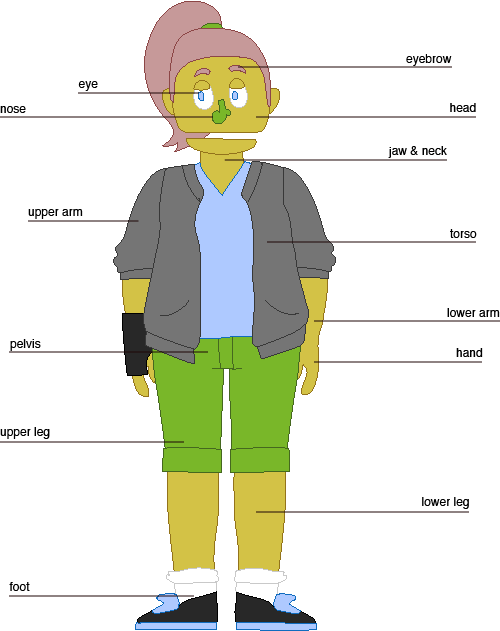
\includegraphics[width=.4\linewidth]{images/character_components}
\caption{Character Components}
\label{fig:character_components}
\end{figure}

\subsubsection{Emotes}
Characters will make use of 2D emotes in order to supplement various aspects of character interaction. These emotes may be triggered through dialogue, yelling contests, or other character interactions. In \ourgame{}, emotes will be represented by 2D spritesheet animations, which will be placed relative to the character's head. Emotes which are triggered through character interactions will play once and then disappear. Emotes may also be tied to a character's state, in which case they play on a loop indefinitely.

\subsubsection{Animations}
Animations will be incorporated using IK skeletal rigs. The character components will be attached to these rigs such that the bones can be manipulated using five end-effectors (control points which bone chains try to reach through rotation). The end-effectors included in the skeletal rig will be one which controls the base of the spine to the top of the head, and four which control the character's limbs. In the animation definition file it will be possible to set the position of end effectors to a percentage of their chain length. This will allow animations to work with characters of various sizes.

An IK chain in \ourgame{} will calculate the position and orientation of connected bones based on the start and end effector positions. In order to do this, the Cyclic Coordinate Descent algorithm is used. The steps of this algorithm are:
\begin{enumerate}
\item{Loop through bones from end to start}
\item{For each bone, rotate from the bone-origin such that the chain's end is as close to the end effector as possible}
\item{If the chain's end is not within a certain threshold, repeat}
\end{enumerate}

Animations will be stored in a JSON file which will contain a reference value for each-end effector position and an array of tween objects. Each tween object will contain the difference in position over a period of time and an interpolation used to define how the position changes during that period of time (e.g. stepped interpolation would cause the end effector to remain in one position, then jump to the next in an instant, whereas linear interpolation would cause the effector to move from one position to the next along the vector which separated them).

\subsection{Room Generation}
At the start of each playthrough, a layout for \ourgame{}'s environment will be generated procedurally. The room generation algorithm starts by selecting approximately 10 scenarios from the game's database for use in the current playthrough. Once these scenarios have been selected, the various characters, items, and room specifications associated with those scenarios must be generated. Once these have been created, they will be grouped into bundles which may each be mapped to a single room at the end of the generation process. For example: one scenario may be defined such that it includes two characters and two room specifications, one of which is tagged with "bathroom". Each character must be placed in one of the specified rooms. A second scenario may be defined such that it includes a single item which must be placed within a container. A third scenario may be defined such that it includes a room specification with the "kitchen" tag. At this stage in the generation algorithm, two bundles will be created. The first bundle will include one room specification with the "kitchen" tag, one character, a single container, and the item; the second bundle will include a room specification with the "bathroom" tag and the other character. This example is visualized in Figure~\ref{fig:room_bundling}. Notably, two of the three rooms specified in the scenarios were merged, producing more potential interactions between the selected scenarios.

\begin{figure}[htb]
 \centering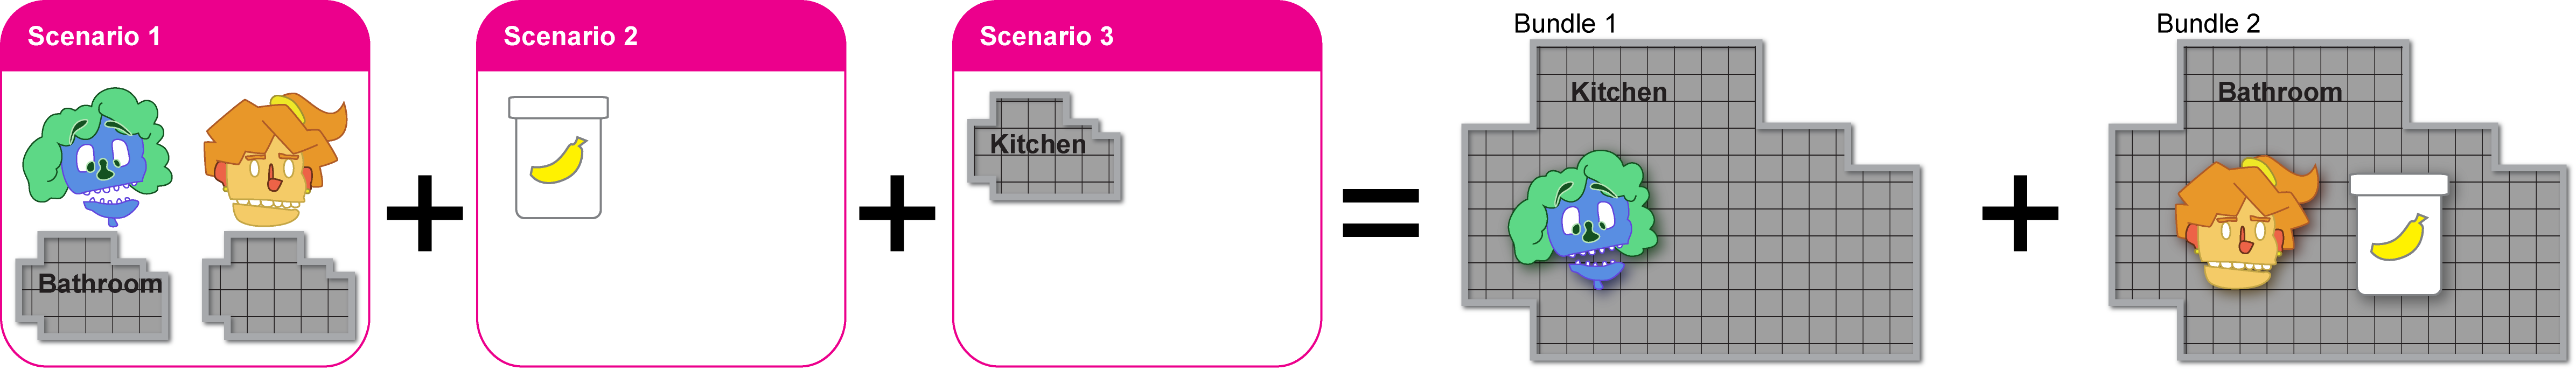
\includegraphics[width=.9\linewidth]{images/bundle}
  \caption{Visualization of room bundling}
  \label{fig:room_bundling}
\end{figure}


Once the scenario contents have been bundled, the layout of the house may be generated. To achieve this, a grid will be created, and subsections of the grid will be selected to create spaces for individual rooms. The size of the grid and individual rooms will be based on the specifications and required room content in each bundle. Inside each subsection, an image will be generated which represents the shape of the room. The room's walls will be created and placed depending on the contours calculated from the room-layout image's pixels. Examples of this procedural generation system can be seen in Figure~\ref{fig:room_generation_example}

\begin{figure}[htb]
 \centering
  \begin{subfigure}{.24\textwidth}
    \centering
    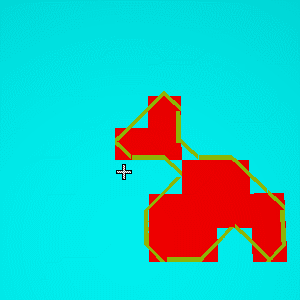
\includegraphics[width=.9\linewidth]{images/maps1}
  \end{subfigure}%
  \begin{subfigure}{.24\textwidth}
    \centering
    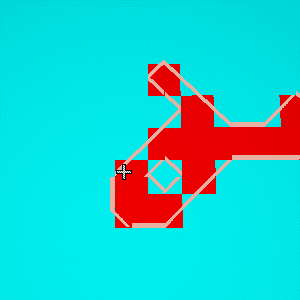
\includegraphics[width=.9\linewidth]{images/maps2}
  \end{subfigure}%
  \begin{subfigure}{.24\textwidth}
    \centering
    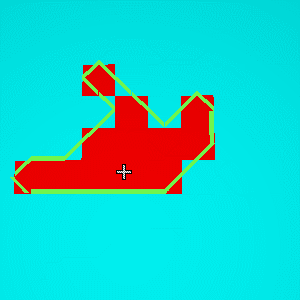
\includegraphics[width=.9\linewidth]{images/maps3}
  \end{subfigure}%
  \caption{Example room generation}
  \label{fig:room_generation_example}
\end{figure}

All objects in a room will be a part of a hierarchy. For example, dining chairs would be parented to a dining table, and a painting would be parented to a wall. To account for this kind of room structure, each room object will have its own list of specifications, which include its bounding box, a tag-based list of possible parents the object can have (e.g. a dining chair can be parented to a dining table), and a list of sides that children can place themselves against (i.e. top, bottom, left, right, front, and back).

 All of the bundle's room objects will try to find parents among themselves, which will include characters, items, furniture/props, and the room walls. Once a parent for a room object has been found, the object will try to align itself along one of the parent's sides, and if there is enough space, the object will position and orient itself beside the parent. If a parent is not found, a random position will be calculated that exists inside the room. A collision check will then be against the rest of the objects in the room, as well as against the room walls.

After the placement of all required room items of the bundle, additional side characters and items required for a scenario will be generated and added to the room using the same placement method as above to ensure there are no collisions or conflicts between characters, items, and furniture.

Once all the rooms have been created, they will then be connected to each other to allow traversal through each room in the map. Each of these connections will be represented in-game by a door item, which may be interacted with by the player in order to move between the different rooms in a layout.

\clearpage
\subsection{3D Art Assets}

\subsubsection{Generative Furniture}
In order to increase the variability of environments that the user will experience while playing \ourgame, most of the environment will be generated at runtime. This will be done by combining components of different parent meshes together to create a new mesh. Parent meshes will be made in Autodesk Maya and be composed of quadrilateral faces (faces with four vertices). The decision to use quadrilateral faces was made because it is easier to deform a mesh with such faces, and these meshes will eventually be deformed in order to give them distorted dimensions and shapes. The parent meshes of a single type of furniture will have similar dimensions in order to make combining their components more easily. While in Autodesk Maya, the parent meshes will be split into components which will be used for furniture generation. Some furniture types may have optional pieces, which do not have to be included in the final mesh. On the components will be at least one connector point which will be used to join the components together. The position of these connector points will be stored in a database on the server. The server will also store other information pertaining to components, including the ID of the component, the type of piece the component is, and what furniture type the component can be used in. When a new play through is initialized, the game will read the scenario files that will be used to populate the game. These files will contain room tags which determine what kind of furniture will be placed inside of that room, as well as information on the furniture components. Using this, the game will select random components that can be used for the specified furniture types, and join the meshes together to create a unique piece of furniture. Optional components can either be included or omitted. When combining furniture components, the root component will be chosen first, as it will most likely determine how many other components are required to complete the piece. Some components will have dependencies, meaning that they cannot be included unless another component has been added to the mesh first. After the components have been combined, a deformer will be used to distort the shape, increasing the variability of furniture, while also helping to add to the strange atmosphere of the game.

\begin{figure}[H]
	\centering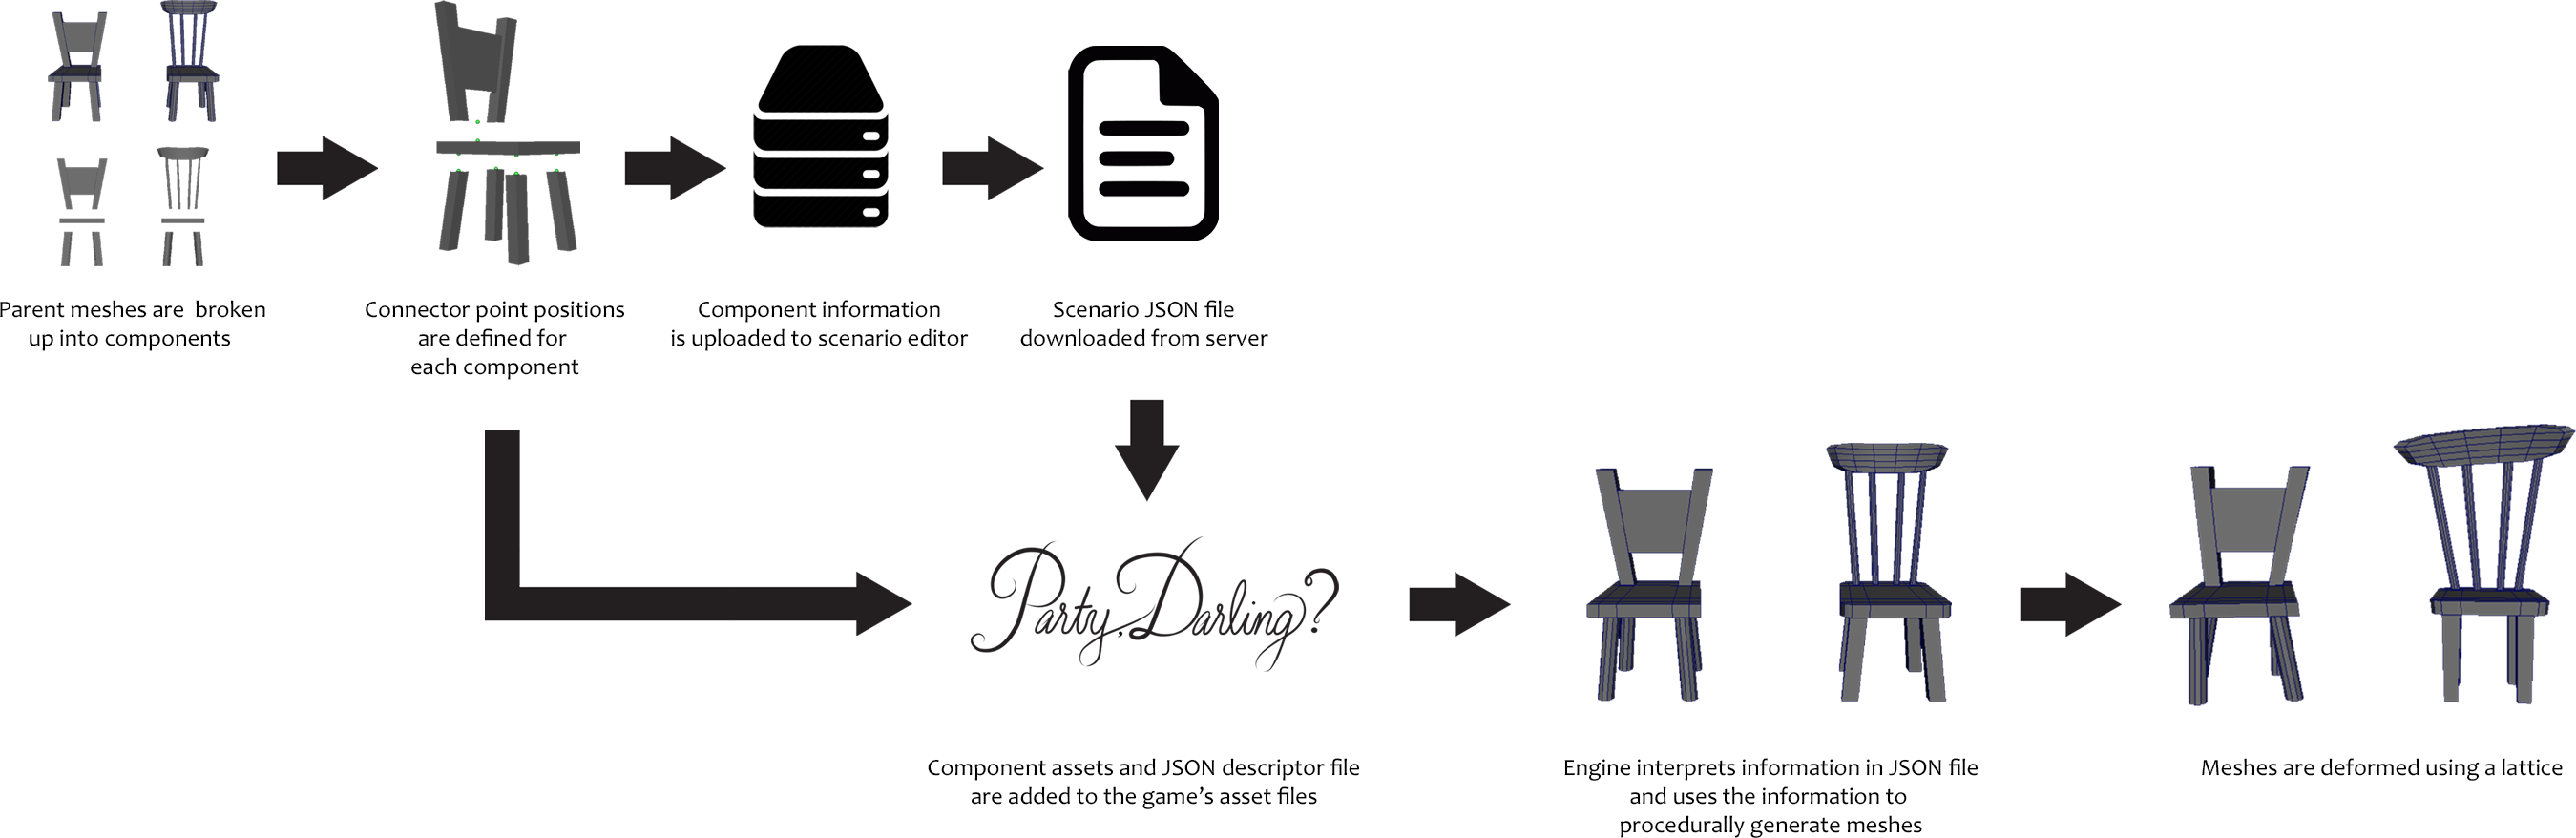
\includegraphics[width=0.8\linewidth]{images/proceduralFurnitureProcess_Diagram}
	\caption{Diagram of the Flow of the Procedural Furniture Generation Process}
	\label{fig:furniture}
\end{figure}

\subsubsection{3D Props}
The game world will be populated with various 3D props. These props will be physics objects, and will be able to collide with the player, as well as other 3D props and environment objects. The props that are included in the world, and their placement, are dictated by the scenario files loaded when the game is initialized. Similar to furniture objects, 3D props will be deformed to change their proportions, adding to the variability of their appearance. These items cannot be placed into a player's inventory, or used in any game play mechanics.

\subsubsection{Deformers}
As stated previously, \ourteam{} will create a few deformers within \ourengine{} which will be used on 3D assets within the game in order to increase their visual variability and to help effect the atmosphere of the game. These will be performed using vertex manipulation in the form of a Lattice deformer.